\documentclass[9pt]{beamer}
\usetheme{CambridgeUS}%establece el tipo de diapositiva
\usepackage[activeacute,spanish]{babel}
\usepackage{graphicx}
\usepackage[utf8]{inputenc}

\title{NotifyMe}
\author{Iván Aveiga \\ Wilson Enriquez \\ Andrés Sornoza}
\institute{Escuela Superior Politécnica del Litoral}


\begin{document}
	\begin{frame}
		\begin{center}
			
\includegraphics[width=0.20\textwidth]{android.png}
		\end{center}
		\titlepage
		\scriptsize
	\end{frame}	
	
	\begin{frame}
		\frametitle{NotifyMe}
			\begin{block}{¿Qué es NotifyMe?}
				NotifyMe es una aplicación que nos permite almacenar nuestras listas de tareas a realizar agrupadas por categorías
				con el valor agregado de que usa el \emph{\textbf{Sistema} de \textbf{Posicionamiento} \textbf{Global}} para alertarnos
				de realizar las tareas cuando estemos cerca de la ubicación geográfica que le hayamos asignado.
			\end{block}
	\end{frame}
	
	\begin{frame}
		\frametitle{NotifyMe}
			\begin{block}{\textbf{ }}

		 \end{block}
	\end{frame}
	
	\begin{frame}
		\frametitle{NotifyMe}
			\begin{block}{\textbf{¿Qué me permite hacer NotifyMe?}}
				\begin{itemize}
					\item \emph{\textbf{Creación, Modificación, Eliminación de Notas}} 
					\item \emph{\textbf{Ubicar las coordenadas de la Nota mediante mapa interactivo}}
					\item \emph{\textbf{Alertar cuando se encuentra en un rango determinado de la ubicación de la(s) tarea(s)}} 				
					\item \emph{\textbf{Uso de categorías, ejemplo: Compras, Ventas, Citas}}
					\item \emph{\textbf{Uso de Lugares, ejemplo: Peluquerías, Agencias de Correo}} *Soportado en futuras versiones.
				\end{itemize}
				\begin{center}
					
\includegraphics[width=0.20\textwidth]{gmaps.png}
					
\includegraphics[width=0.20\textwidth]{gingerbread.png}
				\end{center}
			\end{block}
	\end{frame}
	
	\begin{frame}
		\frametitle{NotifyMe}
			\begin{block}{\textbf{Creación de nota}}
				\begin{center}
					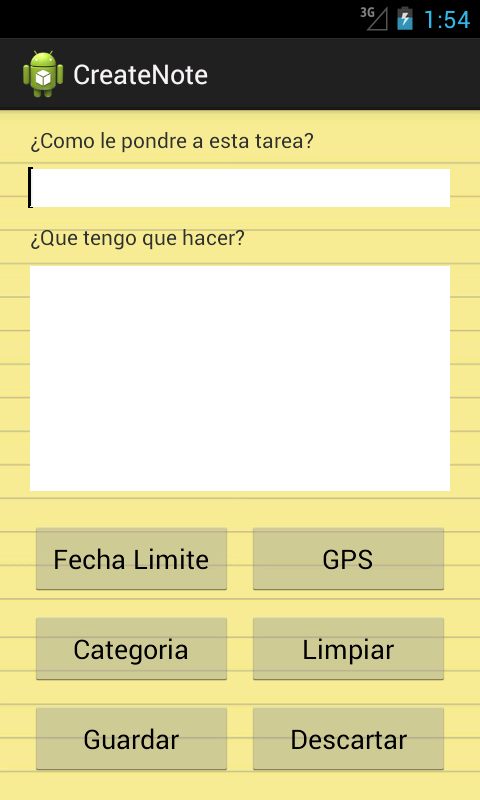
\includegraphics[width=0.20\textwidth]{crearnota.png}

				\end{center}
			 \end{block}
	\end{frame}
	
	\begin{frame}
		\frametitle{NotifyMe}
			\begin{block}{\textbf{Ubicación de nota}}
				\begin{center}
					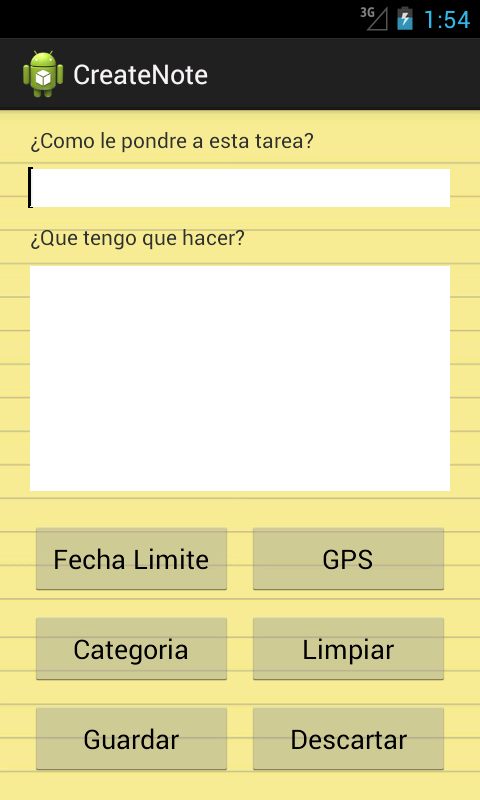
\includegraphics[width=0.20\textwidth]{crearnota.png}

				\end{center}
			 \end{block}
	\end{frame}	
	
	
	\begin{frame}
		\frametitle{NotifyMe}
			\begin{block}{\textbf{Modificación de nota}}
				\begin{center}
					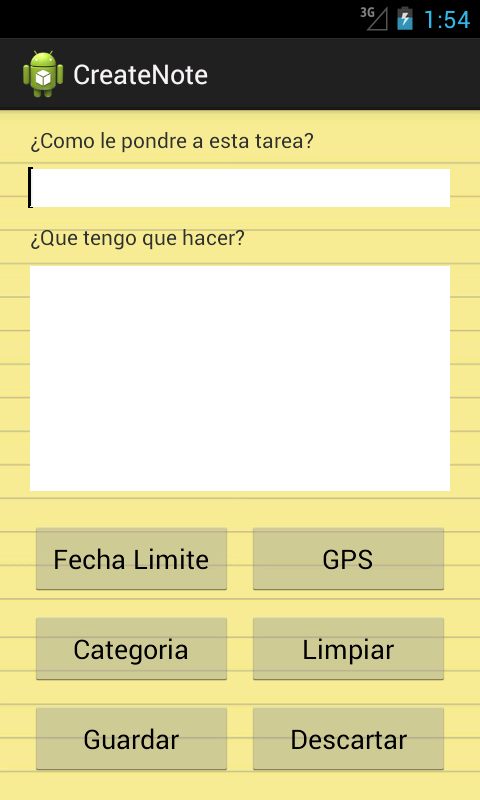
\includegraphics[width=0.20\textwidth]{crearnota.png}

				\end{center}
			 \end{block}
	\end{frame}	
	
	\begin{frame}
		\frametitle{NotifyMe}
		\begin{block}{\textbf{Eliminación de nota}}
			\begin{center}
				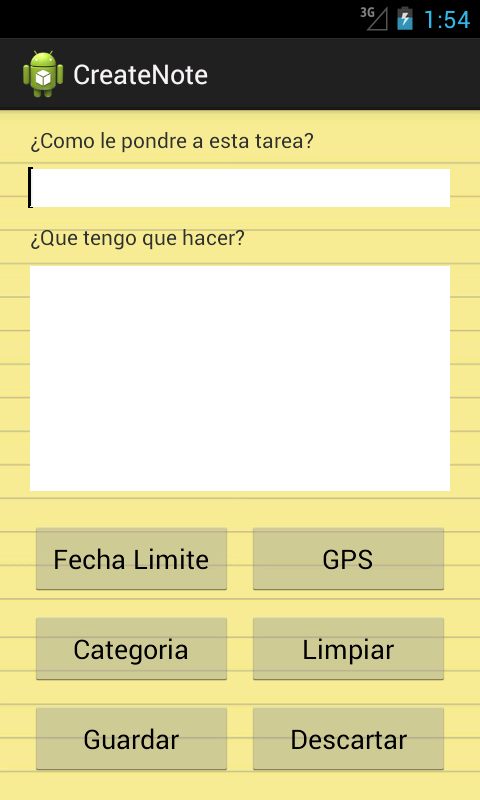
\includegraphics[width=0.20\textwidth]{crearnota.png}
			\end{center}
		 \end{block}
	\end{frame}
		
\end{document}